\section{Related works}

\begin{frame}[plain]
   \sectionpage
\end{frame}

\frame{
   \frametitle{Literature outline}

   \textbf{Overview of HHCP}
   \begin{itemize}
      \item First study from \citeyear{fernandez1974}
      \item Since 2006: +1 new publications per year
      \item At least three major surveys
   \end{itemize}

   \begin{tikzpicture}[overlay]
      \node at (12,1.3) {
\includegraphics[scale=0.1]{fig/fernandez-paper.png}};
   \end{tikzpicture}

   \pause

   \begin{figure}
      \centering
      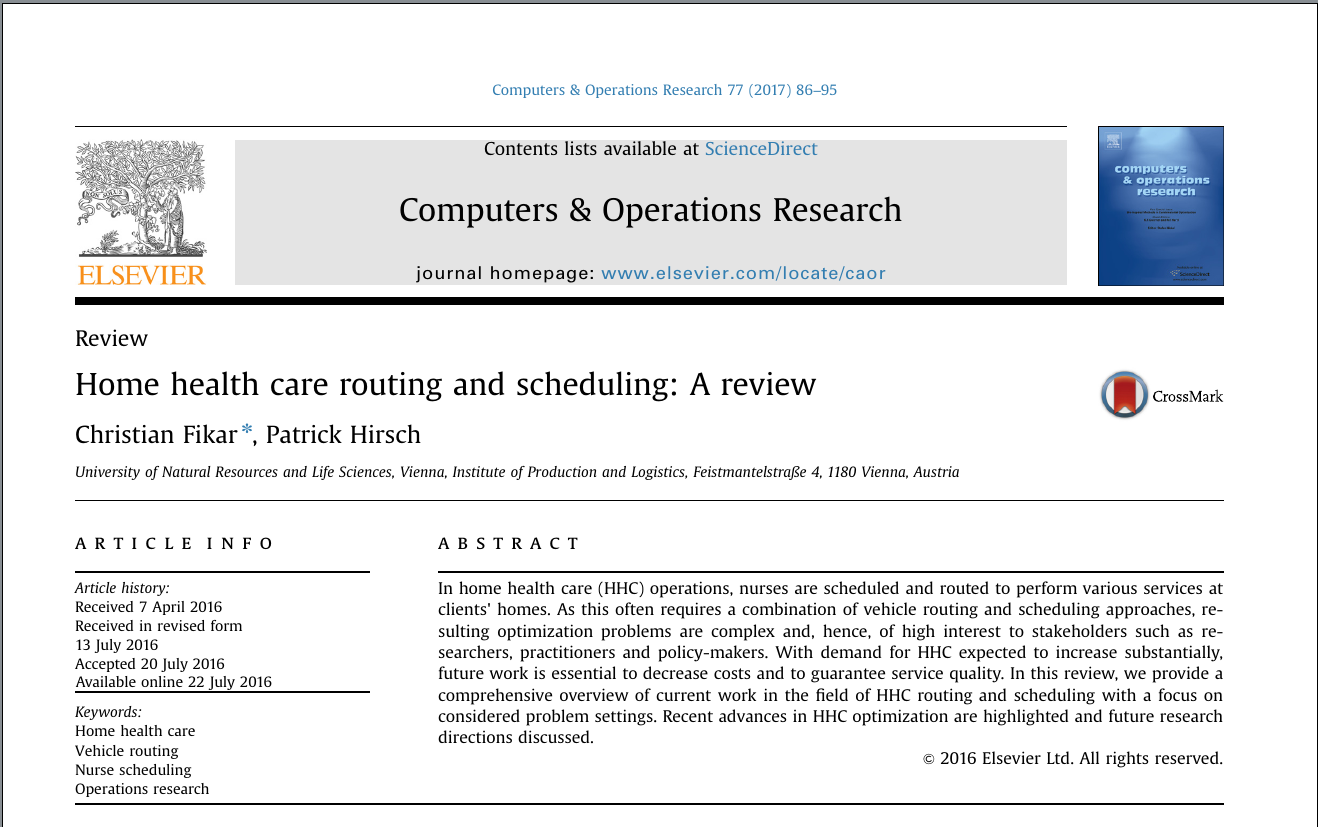
\includegraphics[scale=0.1]{fig/fikar2017-paper.png}
      \hspace{6pt}
      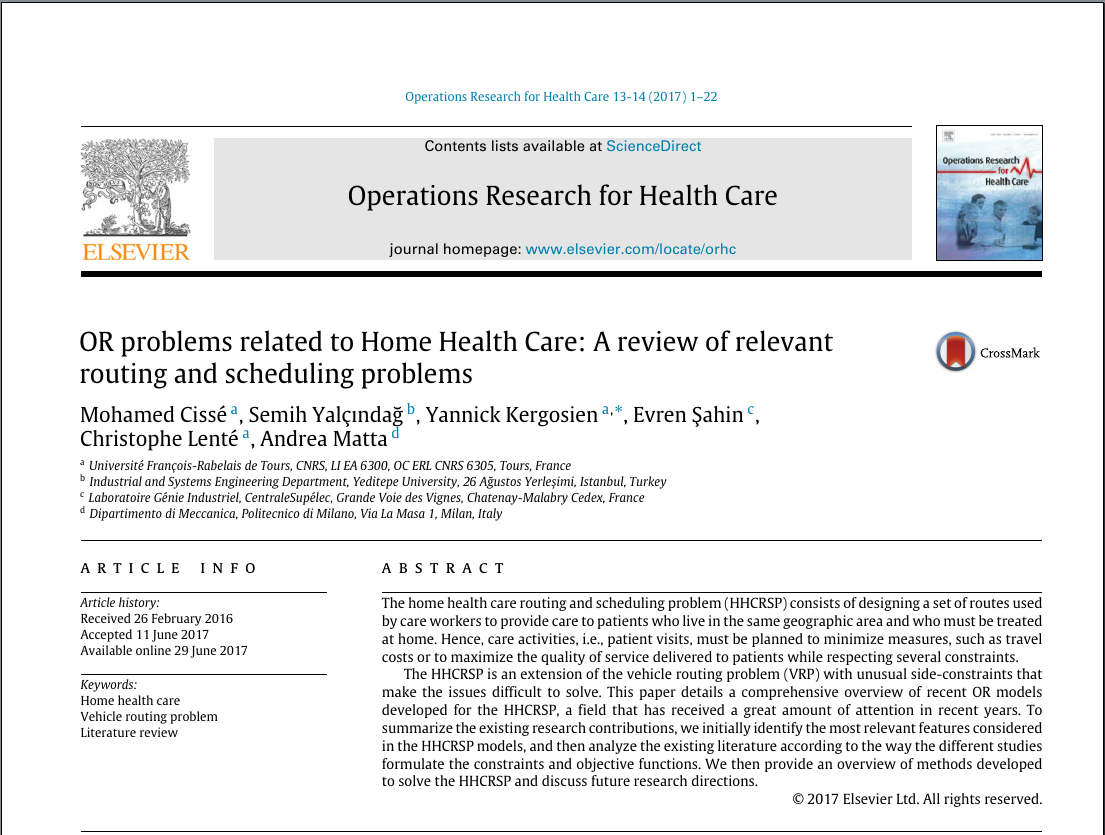
\includegraphics[scale=0.11]{fig/cisse2017-paper.png}
      \hspace{6pt}
      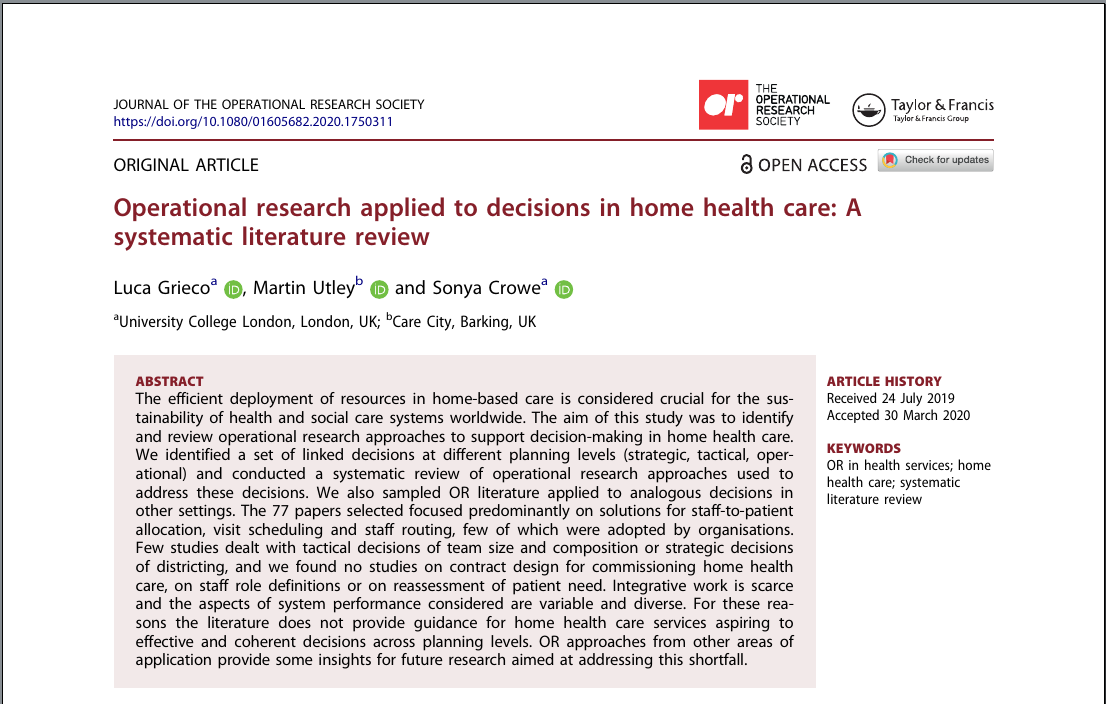
\includegraphics[scale=0.12]{fig/grieco2020-paper.png}
   \end{figure}
}


\frame{
   \frametitle{Literature outline}

   \textbf{In general}
   \begin{itemize}
      \item Most publications approach \emph{only} the routing problem
      \item Focuses on \textbf{home hospitalization}
      \begin{itemize}
         \item Survey: \citet{fikar2017}
         \item Survey: \citet{cisse2017}
      \end{itemize}
      \item Other formats: first care, social care
      \item HC involves \textbf{much more} than routing and scheduling
   \end{itemize}
}

\frame{
   \frametitle{Literature outline}

   \textbf{The HC framework is much more complex}
   \begin{itemize}
      \item Assess epidemiological profile of potential patients to:
      \begin{itemize}
         \item Choice of service types offered
         \item Assessment of visit frequency
         \item Hiring of personnel (staffing)
         \item Routing (caregivers), and visit scheduling (patients)
      \end{itemize}
   \end{itemize}

}

\frame{
   \frametitle[plain]{Literature outline}

   \begin{center}
      \begin{adjustbox}{width=0.4\textwidth}

      \begin{tikzpicture}[mindmap, grow cyclic, every node/.style=concept, concept color=orange!40,
      level 1/.append style={level distance=5cm,sibling angle=120},
      level 2/.append style={level distance=3cm,sibling angle=45}]

         \node{  Home (Health) Care Problem}
         child [concept color=purple!50] { node {  Operational planning}
            child { node {Visit scheduling}}
            child { node {Staff routing}}
            child { node {Inventory control}}
         }
         child [concept color=teal!40] { node {  Tactic planning}
            child { node {Admission control}}
            child { node {Fleet assignment}}
            child { node {Staff allocation}}
            child { node {Temporary staff}}
         }
         child [concept color=blue!30] { node { Strategic planning}
            child { node {Facility location}}
            child { node {Districting}}
            child { node {Service type coverage}}
            child { node {Staffing}}
            child { node {Supplier selection}}
            child { node {Fleet assignment}}
         };
      \end{tikzpicture}
      \end{adjustbox}
      \\[2pt]
      \footnotesize
      Source: based on the work of \citet{gutierrez2013}.
   \end{center}
}

\frame{
   \frametitle{Operational planning for the HC}

   \textbf{We also approach the operational planning}
   \begin{itemize}
      \item Basic VRPTW model \citep{cheng1998}
      \item But no consensus regarding a \textit{standard} problem
      \item No standard dataset
   \end{itemize}

   \begin{tikzpicture}[overlay]
   \node (a) at (11.8,1.3) {
      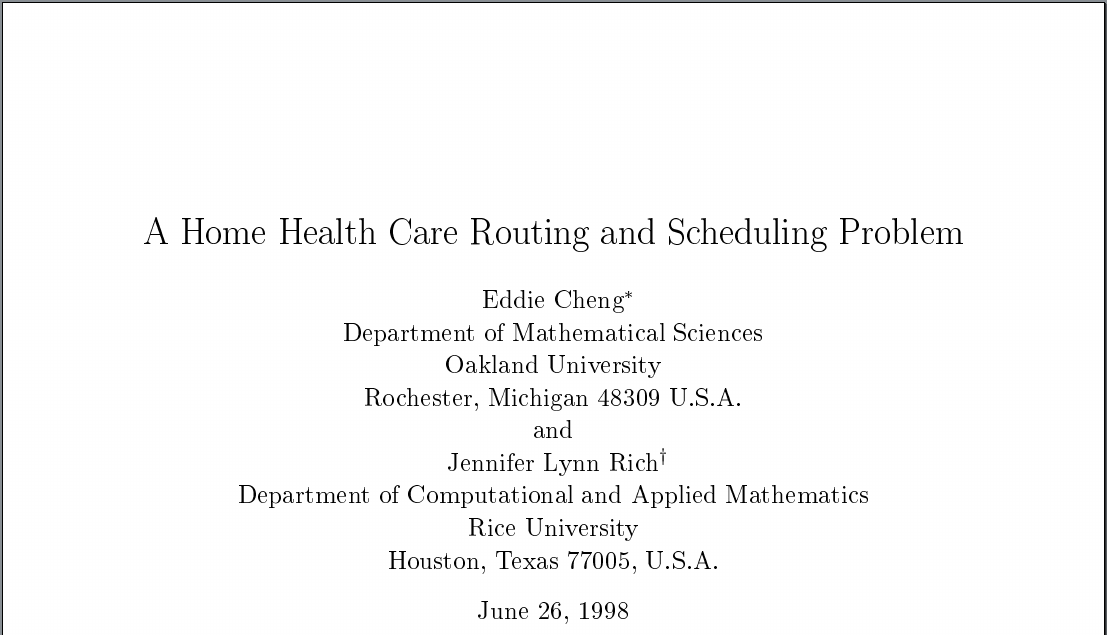
\includegraphics[scale=0.12]{fig/cheng1998-paper.png}
   };
   \end{tikzpicture}
}

%\frame{
%   \frametitle{Operational planning for the HHCP}
%
%   \textbf{Also a rich research subtopic}
%   \footnotesize
%   \begin{itemize}
%      \item Planning horizon length
%      \item Working regulations
%      \item {Preferences}
%      \item {Uncertainty}
%      \item Multiple services types
%      \item Multiple visits, operations synchronization
%      \item \citet{fikar2017}, \citet{cisse2017}, \citet{grieco2020}
%   \end{itemize}
%   \normalsize
%
%   \vspace*{12pt}
%
%   \textbf{Integrated approaches}
%   \footnotesize
%   \begin{itemize}
%      \item Fluctuation demands and temporary hiring \citep{eveborn2006}
%      \item Fleeting and operational planning \citep{fikar2018}
%   \end{itemize}
%   \normalsize
%}